\documentclass[10pt,preprint]{aastex}
%\documentclass[10pt,twocolumn]{article}

%\usepackage[margin=0.85in]{geometry}
%\setlength{\columnsep}{0.2in}
%\documentclass{emulateapj}

\usepackage{verbatim}
\usepackage{color}

\usepackage[normalem]{ulem} % for striking out with \sout
% A comment block

%\newcommand{\comment}[1]{}

% For color
\newcommand{\mpname}[1]{#1_color.eps}
\newcommand{\clraitoff}{red}
\newcommand{\lumblack}{(black)}
\newcommand{\lumblue}{(blue)}
\newcommand{\lumred}{(red)}
\newcommand{\vdisred}{(red-dashed curve)}
\newcommand{\vdisblue}{(blue-solid curve)}

% For bw
%\newcommand{\mpname}[1]{#1.eps}
%\newcommand{\clraitoff}{}
%\newcommand{\lumblack}{}
%\newcommand{\lumblue}{}
%\newcommand{\lumred}{}
%\newcommand{\vdisred}{(dashed curve)}
%\newcommand{\vdisblue}{(solid curve)}

\newcommand{\umag}{$u$}
\newcommand{\gmag}{$g$}
\newcommand{\rmag}{$r$}
\newcommand{\imag}{$i$}
\newcommand{\zmag}{$z$}
\newcommand{\gmr}{$g-r$}



\newcommand{\gammat}{$\gamma_T$}
\newcommand{\gammacross}{$\gamma_\times$}
\newcommand{\deltasig}{$\Delta \Sigma$}
\newcommand{\deltaplus}{$\Delta \Sigma_+$}
\newcommand{\deltacross}{$\Delta \Sigma_\times$}
\newcommand{\deltarho}{$\Delta \rho$}
\newcommand{\movr}{$M(<r)$}
\newcommand{\sigmacrit}{$\Sigma_{crit}$}

\newcommand{\photoz}{photo-z}
\newcommand{\photozs}{photo-zs}

\newcommand{\tlum}{$L^{tot}$}
\newcommand{\tngal}{$N_{gal}^{tot}$}

\newcommand{\lstarlim}{$0.4 L_*$}
\newcommand{\lvir}{$L_{200}$}
\newcommand{\nvir}{$N_{200}$}
\newcommand{\rvir}{$r_{200}^{gals}$}

\newcommand{\ngal}{$N_{gal}$}
\newcommand{\maxbcg}{maxBCG}
\newcommand{\numNgalBins}{12}
\newcommand{\numLumBins}{16}

\newcommand{\tngalAperture}{2$h^{-1}$ Mpc}

\newcommand{\photo}{\texttt{PHOTO}}
\newcommand{\astrop}{\texttt{ASTRO}}
\newcommand{\mt}{\texttt{MT}}
\newcommand{\spectro}{\texttt{SPECTRO}}
\newcommand{\spectroone}{\texttt{SPECTRO1d}}
\newcommand{\spectrotwo}{\texttt{SPECTRO2d}}
\newcommand{\target}{\texttt{TARGET}}

\newcommand{\lenszmax}{0.3}
\newcommand{\lenszmin}{0.05}

\newcommand{\photoversion}{\texttt{v5\_4}}

%\def\eone{e$_1$}
%\def\etwo{e$_2$}
\newcommand{\etan}{e$_+$}
\newcommand{\erad}{e$_\times$}
\newcommand{\eclass}{\texttt{ECLASS}}
\newcommand{\eclasscut}{-0.06}
\newcommand{\gmrcut}{0.7}

\newcommand{\hrs}{$^{\mathrm h}$}
\newcommand{\minutes}{$^{\mathrm m}$}

\newcommand{\ugriz}{$u, g, r, i, z$}
\newcommand{\polarization}{polarization}

\newcommand{\wgm}{$w_{gm}$}
\newcommand{\wgg}{$w_{gg}^p$}
\newcommand{\wmm}{$w_{mm}$}
\newcommand{\xigg}{$\xi_{gg}$}
\newcommand{\ximm}{$\xi_{mm}$}
\newcommand{\xigm}{$\xi_{gm}$}

\newcommand{\numspec}{127,001}
\newcommand{\numspecvlim}{10,277}
\newcommand{\numrand}{1,270,010}
\newcommand{\numspectot}{278,192}
\newcommand{\numvdis}{49,024}
%\newcommand{\numsource}{10,259,949}
% hirata: 
\newcommand{\nummask}{1,815,043}
\newcommand{\numTenMpc}{132,473}
\newcommand{\numThirtyMpc}{101,221}
\newcommand{\numsource}{27,912,891}

\newcommand{\numpairsTenMpc}{2,670,898,177}
\newcommand{\altnumpairsTenMpc}{2.7 billion}
\newcommand{\numpairsThirtyMpc}{14,818,082,122}
\newcommand{\altnumpairsThirtyMpc}{14.8 billion}



\newcommand{\xirmax}{$\xi_{gm}(R_{max})$}


\newcommand{\M}{\textbf{M}}
\newcommand{\X}{\textbf{X}}
\newcommand{\Dx}{\ensuremath{\Delta x}}
\newcommand{\Dy}{\ensuremath{\Delta y}}
\newcommand{\aratio}{\ensuremath{\sigma^2_{psf}/\sigma^2_{gal}}}
%\newcommand{\aratio}{$\sigma^2_{psf}/\sigma^2_{gal}$}
\newcommand{\psf}{PSF}
\newcommand{\snmatch}{\ensuremath{(S/N)_{m}}}
%\newcommand{\Rshear}{\ensuremath{R_{sh}}}
\newcommand{\Rshear}{\ensuremath{\mathcal{R}}}
\newcommand{\rfracerr}{\ensuremath{\Delta \Rshear/\Rshear}}

\newcommand{\downloadURL}{{\tt http://www.sdss3.org/dr8/data\_access.php\#VAC}}
\newcommand{\datamodelURL}{{\tt http://data.sdss3.org/datamodel/files/BOSS\_PHOTOOBJ/photoz-weight/pofz.html}}
\def\eps@scaling{1.0}% 

%\slugcomment{Last revision \today}
%\shortauthors{Sheldon}
%\shorttitle{Gaussian Mixtures for Shape Measurement}

\begin{document}

\fontsize{10pt}{1}
\selectfont

%\footnotesize
%\scriptsize

\title{Gaussian Mixtures for Shape Measurement}

\author{
Erin S. Sheldon\altaffilmark{1}
}

\altaffiltext{1}{Brookhaven National Laboratory, Bldg 510, Upton, New York 11973}


\begin{abstract}

GMix

\end{abstract}

\section{Gaussian Mixtures} \label{sec:gmix}

The two dimensional Gaussian intensity function is defined as
\begin{equation}
G = \frac{p}{2 \pi \sqrt{|\M|} } ~~ \textrm{exp}\left( -\frac{1}{2} \X^T \M^{-1} \X \right)
\end{equation}
where \M\ is the covariance matrix
\begin{equation}
\M = \left( \begin{array}{cc}
\M_{xx} & \M_{xy} \\
\M_{xx} & \M_{yy} \end{array} \right)
\end{equation}
and \X\ is the position vector relative to the mean of the Gaussian
\begin{equation}
\X = \left( \begin{array}{c}
\Dx \\
\Dy \end{array} \right),
\end{equation}
where we have defined the positions relative to the center $(x_0,y_0)$
as $\Delta x=(x-x_0)$ and $\Delta y=(y-y_0)$.

Under convolution with a Gaussian point-spread-function (\psf) $P$ we measure an
observed model intensity profile
\begin{equation}
G_o = G * P
\end{equation}
In this case the covariance matrices simply add
\begin{equation}
\M_o = \M + \M_{P}
\end{equation}

We can fit a number of gaussians to a galaxy or star image.  There is 
no guarantee this will be a good representation, as sums of Gaussians
do not form a complete set of functions.   This model can be represented
as
\begin{equation}
I = \sum_{i=1}^{N_{g}} p_i G_i
\end{equation}

If the \psf\ is also represented as a sum of gaussians, then the observed
light intensity profile can be modeled as
\begin{eqnarray} \label{eq:postpsf}
I_o & = & \sum_{i=1}^{N_{g}} p_i \sum_{j=1}^{N_{P}} G_i * P_j \\
    & = & \sum_{i=1}^{N_{g}} p_i \sum_{j=1}^{N_{P}} \frac{1}{2 \pi \sqrt{|\M_o|} } ~~ \textrm{exp}\left( -\frac{1}{2} \X^T \M_o^{-1} \X \right) \\
%    & = & \sum_{i=1}^{N_{g}} p_i \sum_{j=1}^{N_{P}} \frac{1}{2 \pi \sqrt{|\M + \M_P|} } ~~ \textrm{exp}\left( -\frac{1}{2} \X^T (\M+\M_P)^{-1} \X \right) \\
\end{eqnarray}
where the $P_j$ are normalized such that the integral over
the plane is unity
\begin{equation}
\int \sum_{j=1}^{N_{P}} P_j dA = 1.
\end{equation}

A Gaussian defined as above has 6 parameters, $x_0, y_0, \textrm{M}_{xx},
\textrm{M}_{xy}, \textrm{M}_{yy},$ and an intensity $p$.  We define a general gaussian
mixture as a set of $N_g$ Gaussians.  Such a Gaussian 
mixture has $6 N_g$ total parameters.

\subsection{Alternative Parametrization}

An alternative parametrization of the covariance matrix is in
terms of the ellipticity parameters and size
\begin{equation}
\M = \frac{T}{2}\left( \begin{array}{cc}
1+e_1 & e_2 \\
e_2 & 1-e_1 \end{array} \right),
\end{equation}
where the ellipticity and size $T$ are defined in terms
of the elements of the covariance matrix as
\begin{eqnarray}
T & = & M_{xx} + M_{yy} \\
e_1 & = & \frac{M_{xx}-M_{yy}}{T}  = e ~ \textrm{cos} (2 \theta) \\
e_2 & = & \frac{2 M_{xy}}{T}  = e ~ \textrm{sin} (2 \theta) \\
e & = & \sqrt{e_1^2 + e_2^2},
\end{eqnarray}
where $\theta$ is the position angle relative to the coordinate system. 
The components 
$e_1$ and $e_2$ are bounded within
$[-1,1]$ and total ellipticity $e$ is within $[0,1]$.  Note in this
parametrization, the argument of the exponential is
\begin{equation}
\frac{1}{2} \X^T \M^{-1} \X = \frac{\Dx^2 (1-e_1) - 2 \Dx \Dy~e_2 + \Dy^2 (1+e_1)}{T (1-e^2)}
\end{equation}


\subsection{Co-elliptical Gaussians}

We will find it useful to use co-elliptical Gaussians; Gaussians with
proportional covariance matrices.  In this case, the dimensionality for $N_g$
Gaussians is reduced from $6 N_g$ to $2 N_g + 4$.  We parametrize this model
with $x_0, y_0, e_1, e_2, T_{max}, f_{i}, p_{i}$ where $T_{max}$ represents
the largest Gaussian and $f_{i} = T_{i}/T_{max}$ is the relative size of
Gaussian $i$, and $p_i$ is the intensity in Gaussian $i$.


%\section{Examples}

%In this section we show some fits to example profiles.

%\subsection{Exponential Disk}

%An exponential disk can be represented reasonably well by three Gaussians
%as shown in Fig. 
%\ref{fig:expcmp}

%\begin{figure}[t] \centering
% \centering 
% \includegraphics[scale=0.7]{figures/test-opt-exp.eps}

% \caption{A fit to an exponential disk using three Gaussians.}
% \label{fig:expcmp}

%\end{figure}



\section{Fitting for the Pre-\psf\ Object}

In order to fit for the pre-\psf\ object, we first fit the \psf\ to a gaussian
mixture.  Then, for a given set of object parameters, we generate a model that
is convolved with this \psf\ according to equation \ref{eq:postpsf} and compare
with the image.  We then search for a set of parameters that gives the best fit
in a $\chi^2$ sense.  

Note both the object and \psf\ are convolved with the pixel response function.
This pixelization is accounted for when fitting a Gaussian mixture model to the
observed \psf.  Thus when using equation \ref{eq:postpsf} to generate the
model, we are fitting for parameters of an object {\it before} convolution with
the \psf, including the pixel response.  We call these the parameters of the
pre-\psf\ model.

\section{Recovering Shear from Shapes}

We use our models to fit for the ellipticity of each object.  We can then
average these shapes to estimate a mean shear as outlined in \citet{bern02}.
Key to this is the application of an average ``shear response'', \Rshear.  The
shear response tells us how an image of a given ellipticity responds to an
applied shear.  For an average shear we can also measure an average response.
For this work we use an unweighted estimator for the average ellipticity and
the response \citep[see e.g.  Equation 5.11,][]{bern02}:
\begin{equation} \label{eq:shearest}
\langle \gamma_i \rangle  = \frac{\langle e_i \rangle}{2 \langle 1 - \frac{1}{2} e^2 \rangle } \equiv
  \frac{\langle e_i \rangle}{2 \Rshear} 
\end{equation}
\noindent Errors in the average total square ellipticity will, to leading
order, result in a fractional error in the shear of $\sim$ \rfracerr = 
0.5 $\Delta e^2/(1-0.5 e^2)$.

\section{Simulations} \label{sec:sim}

We generated a set of mock galaxy and \psf\ images for test purposes.  We use
three different elliptical galaxy models: Gaussian, exponential, de
Vaucouleurs' model \citep{devauc1948}.  We also use three different \psf\ models:
Gaussian, double Gaussian, and a \psf\ representing atmospheric turbulence (XXX
cite kaiser or other).

For the special case of a Gaussian galaxy convolved by Gaussian \psf, the
convolution is performed analytically and only convolution with the pixel
response is done numerically.  

For non-Gaussian models we use a Fast Fourier Transform (FFT) convolution (XXX
cite FFT and scipy).  We first generate the images on a super-fine mesh. We
then FFT the image, multiply the image by the \psf\ in Fourier space, and
transform back. Finally, we re-sample at the desired pixel scale.  Using this
fine mesh is a way to perform accurate convolution with the pixel response, but
more importantly it is necessary for accurate FFTs.  We performed convergence
tests for each type of profile to determine the sampling required to obtain
accurate results.

Gaussian and turbulent \psf s have closed mathematical forms in Fourier space.
When convolving a Gaussian with a non-Gaussian object, or when using a
turbulent \psf, we generate the \psf\ in Fourier space directly.

\subsection{Simulation Parameters}

For all simulation runs we use a single \psf\ and galaxy type with different
orientations and noise properties.  The relevant parameters for each simulation
are the galaxy ellipticity $e$, the ratio of \psf\ area to galaxy area \aratio,
the signal to noise ratio S/N, and the applied shear $\gamma$.

The area ratio \aratio\ is defined as the ratio of the unweighted second
moments of \psf\ and object.  As such, it does not correspond directly to the
area ratio as determined by weighted moments or of any particular fitting
routine in the presense of noise.  For very extended objects such as \devauc\
profile, it may be impossible to recover this size at low S/N.  We use \aratio\
simply as a label.

Similarly, the S/N is defined arbitrarily as the ``optimally matched''
detection S/N.  This matched S/N is a derived from the square image intensity
$I_i$ over pixels $i$
\begin{equation}
\left(\frac{S}{N}\right)^2_{match} = \frac{1}{n} \sum_{i} I_i^2.
\end{equation}
where we have assumed unit pixels and $n$ is a uniform variance per pixel.
This can be shown to be the maximal measure of detection S/N under the
assumptions of sky-noise limited images and uniform noise \citep{plazasthesis}.
It is important to think of this simply as a, fairly arbitrary, label.  The
unweighted S/N is typically much smaller, and the ratio between the optimal and
unweighted S/N depends dramatically on the galaxy profile and aperture.

\subsection{Applied Shear} \label{sec:sim:shear}

For each set of images, we add a constant, weak shear of order 0.01.  We do not
attempt to recover spatially varying shear.  We applied the shear using the
addition rule for distortions as given by Equation 2.6 of
\citet{Escude91}. A galaxy with intrinsice shape $(e_1,e_2)$, when
sheared with a distortion $(\delta_1, \delta_2)$ will have an observed
ellipticity
\begin{eqnarray}
e_1^o  & = & \frac
{e_1 + \delta_1 + \delta_2/\delta^2\left[1 - \sqrt{1-\delta^2}\right]\left( \delta_1 e_2 - \delta_2 e_1\right)}
{1 + \delta_1 e_1 + \delta_2 e_2 } \\
e_2^o  & = & \frac
{e_2 + \delta_2 + \delta_1/\delta^2\left[1 - \sqrt{1-\delta^2}\right]\left( \delta_2 e_1 - \delta_1 e_2\right)}
{1 + \delta_1 e_1 + \delta_2 e_2 },
\end{eqnarray}
where, again, superscript $o$ denotes ``observed'' quantities.

One can transform between shear and $\delta$ using the rules given by
\citet{bern02} in Section 2.2; note however, that we use the ellipticity 
$e$ interchangeably with distortion $\delta$, where as \citet{bern02} define
$e$ as $1-q$ where $q$ is the axis ratio.

\subsection{Models}

\section{Types of Tests}

\subsection{Ring Tests of Shear Recovery}

We place pairs of images at exactly 90 degree relative position angle across
the full range of position angle $2 \theta \in [0,360)$.  When using this
so-called ``ring test'' \citep{Nakajima2007}, the noise from the intrinsic
galaxy shape cancels exactly in the absence of noise.  Since this ``shape
noise'' will dominate the noise in many cases, the ring test reduces the number
of simulated images needed to accurately test shear recovery for our algorithm.

\subsection{Total Ellipticity Recovery}

We generate models with a range of intrinsic total ellipticities and test the
recovery as a function of resolution and S/N.  This test is relevant because we
use the average square total ellipticity to calculate the shear response
\Rshear, which is used to convert the a mean ellipticity to a
mean shear according to Equation \ref{eq:shearest}.

\section{Gaussian Object and Gaussian \psf}

We start with a single Gaussian galaxy convolved with a single Gaussian \psf,
which is a natural fit for the Gaussian mixture model.  

\subsection{Shear Error vs. Galaxy Ellipticity}

In figure \ref{fig:set-e-gg02} we show a set of ring tests as a function of
intrinsic galaxy ellipticity.  In each panel we show simulations with a
different S/N.  Within each panel, the curves represent different values of the
\psf\ to galaxy area ratio \aratio.  In the bin with S/N = 10 we see dependence
of the shear error on ellipticity and \aratio.  For S/N = 20 we see reduced
dependence on ellipticity and the error is of order $10^{-3}$, even for the
highest \aratio.  For higher S/N the error is generally within the noise of our
simulation.

\begin{figure}[t] \centering
 \centering 
 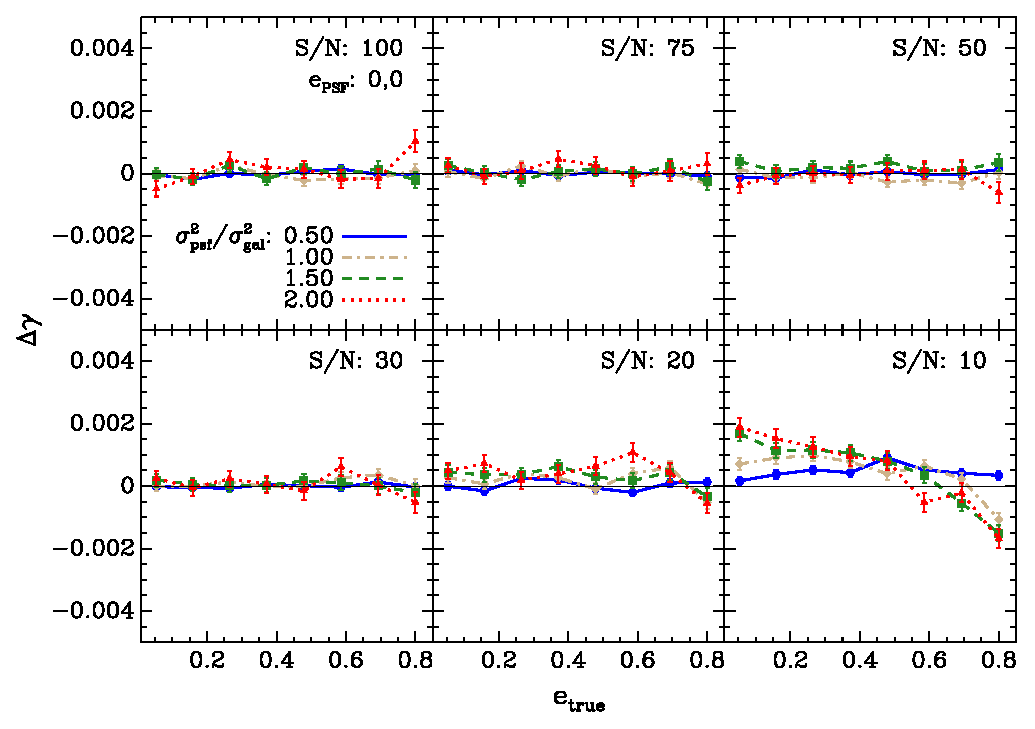
\includegraphics[scale=1]{figures/set-e-gg02-yr-0.005-0.005-vs-e.eps}

 \caption{Shear error vs galaxy input ellipticity for round gaussian \psf\ and
 gaussian galaxies. The intrinsic shear is 0.01.  In this plot we show
 $\gamma_1$; we find similar results for $\gamma_2$.  \label{fig:set-e-gg02}}

\end{figure}

%In Figure
%\ref{fig:gg04r09} we show the fractional error in the estimated shear response
%\rfracerr\ as a function of the galaxy ellipticity for very low noise
%simulations (S/N=$10^6$).  We show a curve for various values of the area ratio
%\aratio.  For this now noise simulation we recover the shear response to better
%than a part in $10^4$ for all values of ellipticity and \aratio.


\subsection{Shear Error vs. Galaxy S/N}

Next we explore the shear error as a function of S/N and fixed ellipticity.  We
use more trials for each point to better access the dependence of error on S/N.

XXX do the other two ellipticities and make new multiplotter for that
where we just show g1 and all three ellipticities.

\begin{figure}[h] \centering
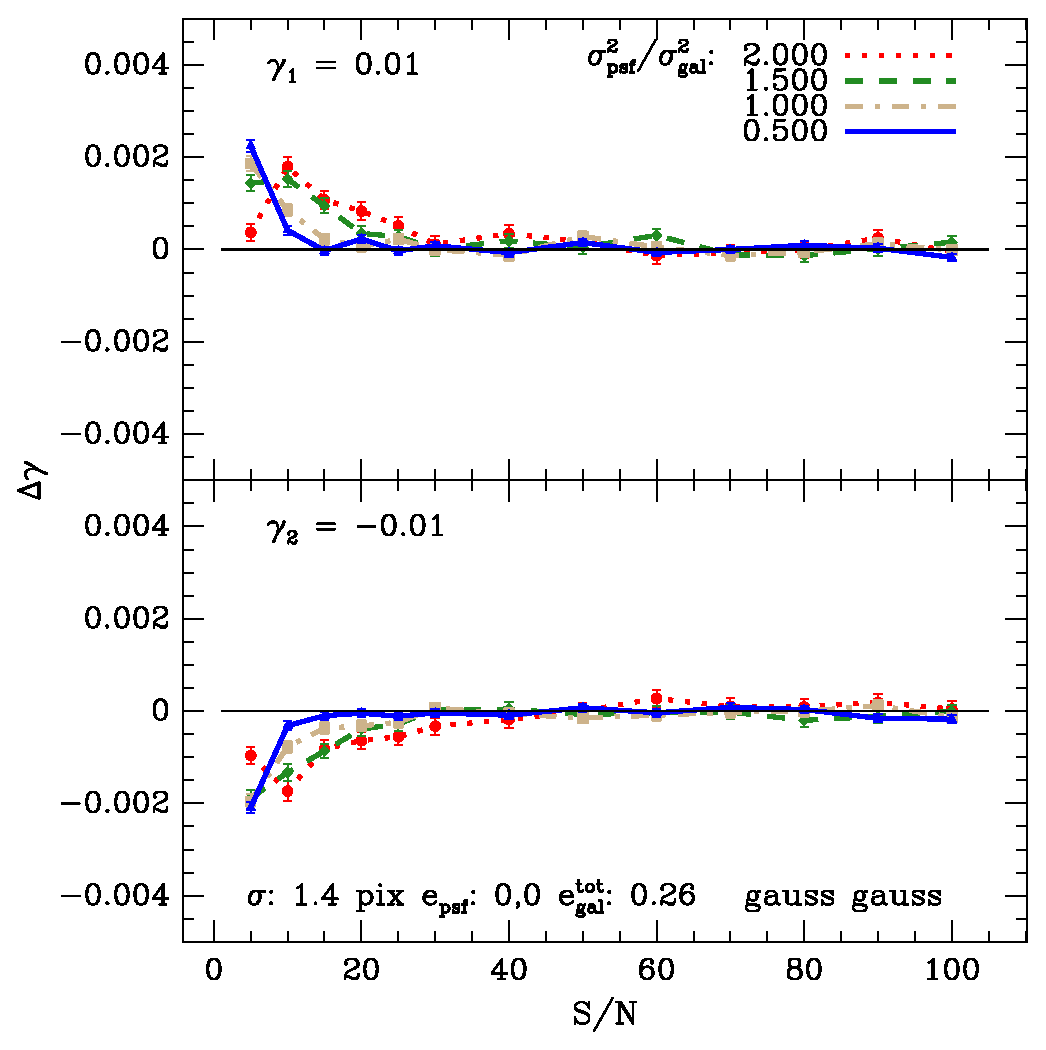
\includegraphics[scale=0.7]{figures/gmix-fit-gg05r14-yr-0.005-0.005-diff.eps}

 \caption{Shear error vs matched S/N for round gaussian \psf\ and gaussian
 galaxies. The intrinsic shear is shown in the upper left corner of each panel.
 These galaxies have total ellipticity 0.33.
 \label{fig:gg05r14}}

\end{figure}


\section{Exponential Object and Turbulent Atmospheric \psf}

We find that exponential disk galaxies are well represented by three guassian
components.  We find that the turbulent \psf\ is also well represented with
three gaussians.

\subsection{Shear Error vs. Galaxy Ellipticity}

%In figure \ref{fig:set-e-et01} we show a set of ring tests as 
%in \ref{fig:set-e-gg01}

XXX These sims need to finish running

%\begin{figure}[t] \centering
% \centering 
% \includegraphics[scale=1]{figures/XXX}

% \caption{Shear error vs galaxy input ellipticity for for round gaussian \psf\
% and gaussian galaxies. The intrinsic shear for $\gamma_1$ is 0.01.  This plot
% shows $\gamma_1$; we find similar results for $\gamma_2$.  The curves in each
% panel are not independent, but accumulate from larger to smaller galaxies.
% Errors bars are shown only for the largest galaxies.
% \label{fig:set-e-gg01}}

\subsection{Shear Error vs. Galaxy S/N}

\begin{figure}[t] \centering \centering
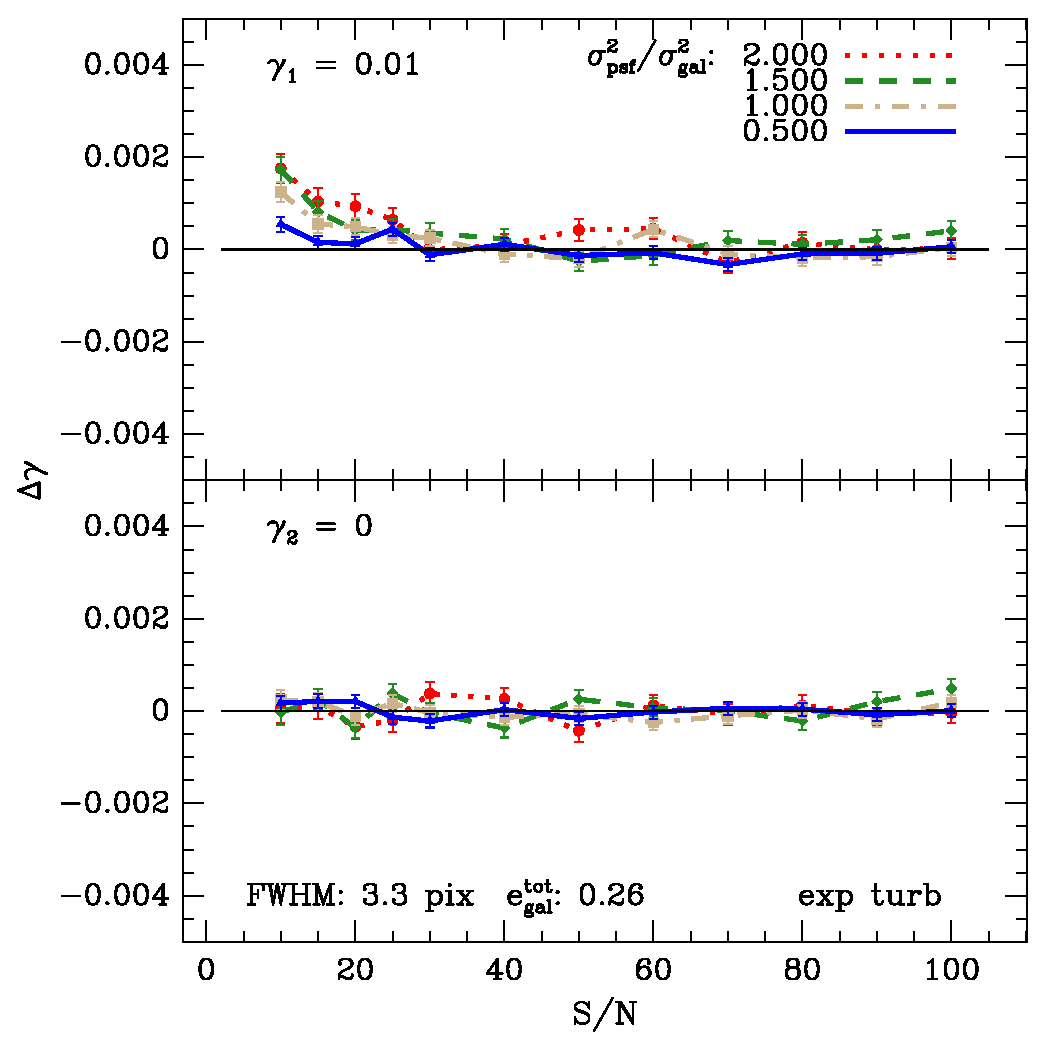
\includegraphics[scale=0.7]{figures/gmix-fit-et06r02-yr-0.005-0.005-diff.eps}

 \caption{Shear error vs matched S/N for turbulent atmospheric \psf\
 and exponential galaxies. The intrinsic shear is shown in the upper left of
 each panel.  These galaxies have total ellipticity 0.33.
 \label{fig:et06r02}}

\end{figure}

\section{\devauc\ Object and Turbulent Atmospheric \psf}

We find that exponential disk galaxies are well represented by four guassian
components.

\subsection{Shear Error vs. Galaxy Ellipticity}

%In figure \ref{fig:set-e-et01} we show a set of ring tests as 
%in \ref{fig:set-e-gg01}

XXX These sims need to finish running

%\begin{figure}[t] \centering
% \centering 
% \includegraphics[scale=1]{figures/XXX}

% \caption{Shear error vs galaxy input ellipticity for for round gaussian \psf\
% and gaussian galaxies. The intrinsic shear for $\gamma_1$ is 0.01.  This plot
% shows $\gamma_1$; we find similar results for $\gamma_2$.  The curves in each
% panel are not independent, but accumulate from larger to smaller galaxies.
% Errors bars are shown only for the largest galaxies.
% \label{fig:set-e-gg01}}

\subsection{Shear Error vs. Galaxy S/N}

\begin{figure}[t] \centering \centering
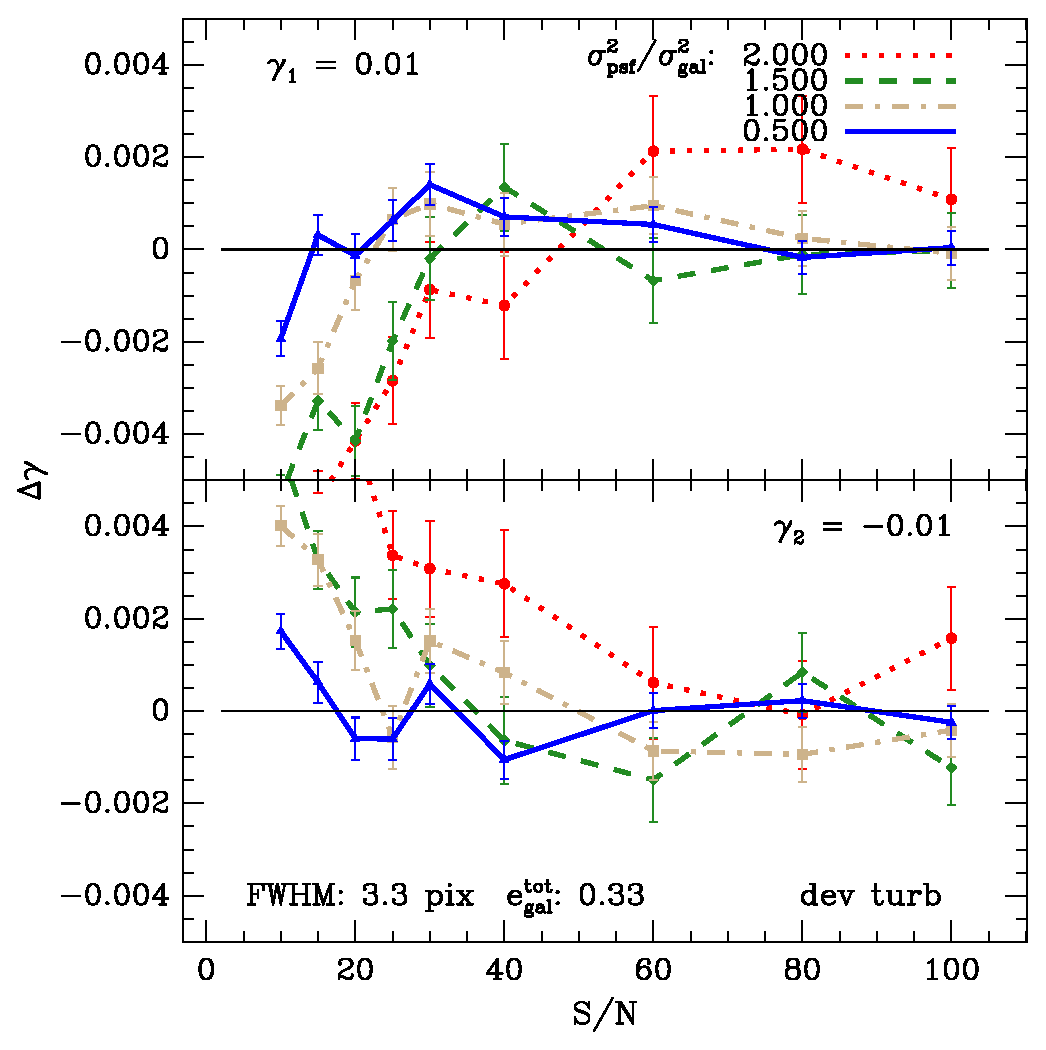
\includegraphics[scale=0.7]{figures/gmix-fit-dt03r05-yr-0.005-0.005-diff.eps}

 \caption{Shear error vs gaussian weighted S/N for turbulent atmospheric \psf\
 and \devauc\ galaxies. The intrinsic shear is shown in the upper left of each
 panel.  These galaxies have total ellipticity 0.33.  \label{fig:dt03r05}}

\end{figure}


\section{Calibration and Additive Errors}

In this section we further explore calibration and additive errors.  By
exploring the shear error as a function of true shear and \psf\ ellipticity, we
can isolate the calibration and additive errors, as defined in the following
equation:
\begin{equation}
\langle \gamma \rangle = m\times \gamma_{true} + c
\end{equation}
The calibration error is related to the slope as $m-1$.  The additive error is
present even at zero shear, and can be caused by incomplete correction for the
effects of an elliptical \psf.  We will isolate the calibration error by first
exploring round \psf s at different shear values.  We will isolate the additive
error by setting the shear to zero and testing the shear recover at different
\psf\ ellipticities.

\subsection{Calibration Errors for Exponential Objects and Atmospheric Turbulence}

In this section we explore calibration errors for objects with exponential
profiles convolved with a \psf\ representing a turbulent atmosphere.  Because
this model is purely round, we cannot fully explore additive errors, but we
will demonstrate that at zero shear we detect no significant additive component.


\begin{figure}[p] \centering
 \centering 
 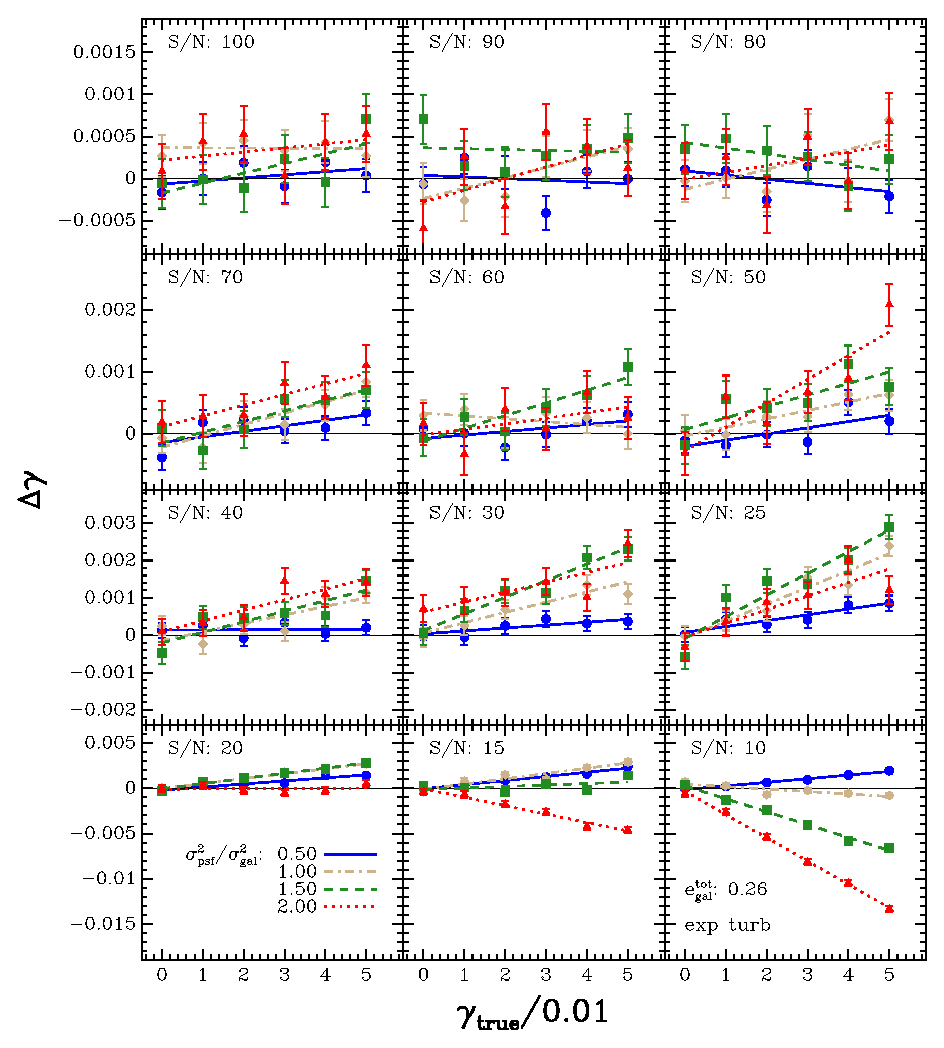
\includegraphics[scale=1.1]{figures/set-s2n-et01-vs-shear.eps}

 \caption{Shear error vs true shear for atmospheric turbulence \psf s
 and exponential galaxies.  Note the vertical scale is different for each row
 of plots.  The over-plotted curves are the best-fitting linear model.}
 \label{fig:etdiffvsshroundpsf}

\end{figure}


\begin{figure}[t] \centering
 \centering 
 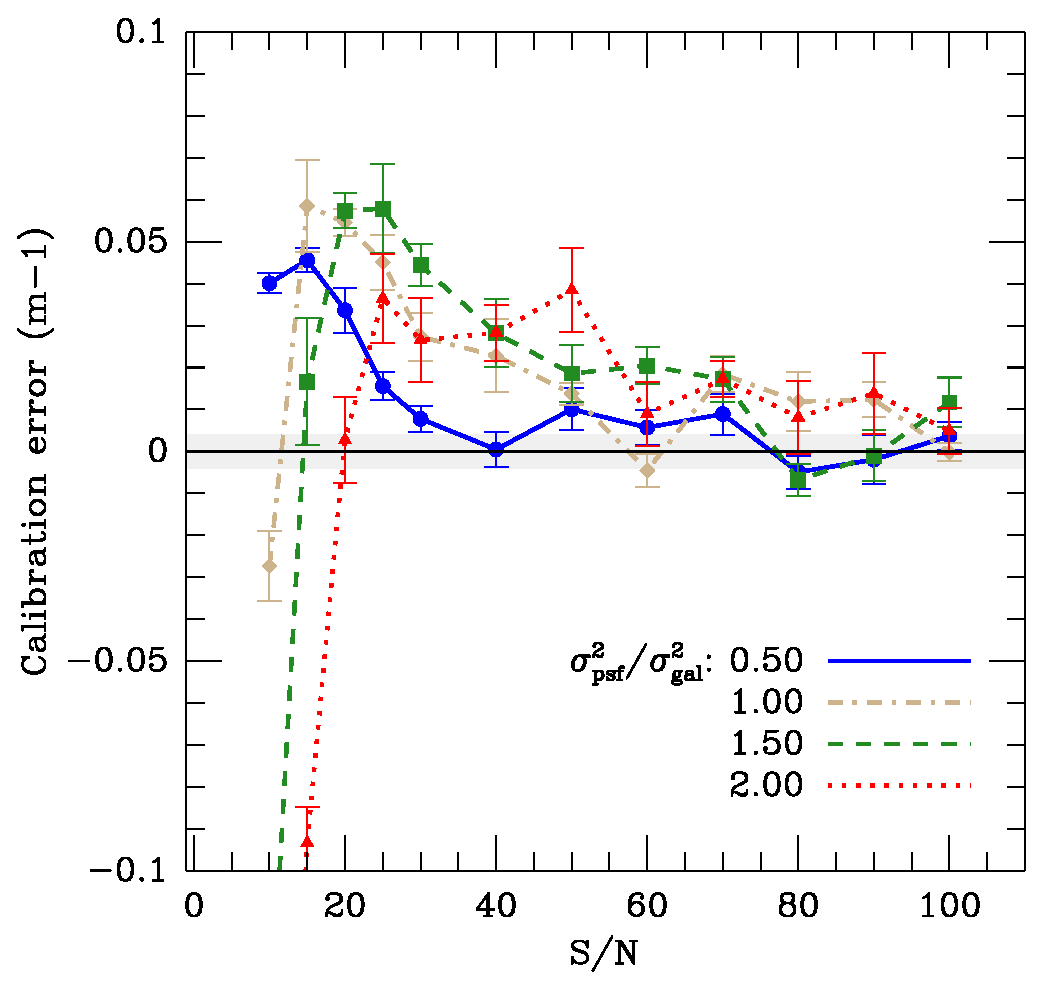
\includegraphics[scale=0.65]{figures/set-s2n-et01-m-vs-shear.eps}

 \caption{Calibration error error as a function of matched S/N for atmospheric
 turbulence  \psf s and exponential galaxies.  The calibration error is
 $\Delta \gamma/\gamma = (m-1)$, where $m$ is the linear slope of the fits shown in
 Figure \ref{fig:etdiffvsshroundpsf}.  The grey region represents the 
 maximum calibration error allowed by Dark Energy Survey science
 requirements.  The matched S/N is the maximal possible S/N measure.  Any real
 world S/N estimate will be considerably lower for these objects.} 

 \label{fig:etcaliberr}

\end{figure}

\begin{figure}[t] \centering
 \centering 
 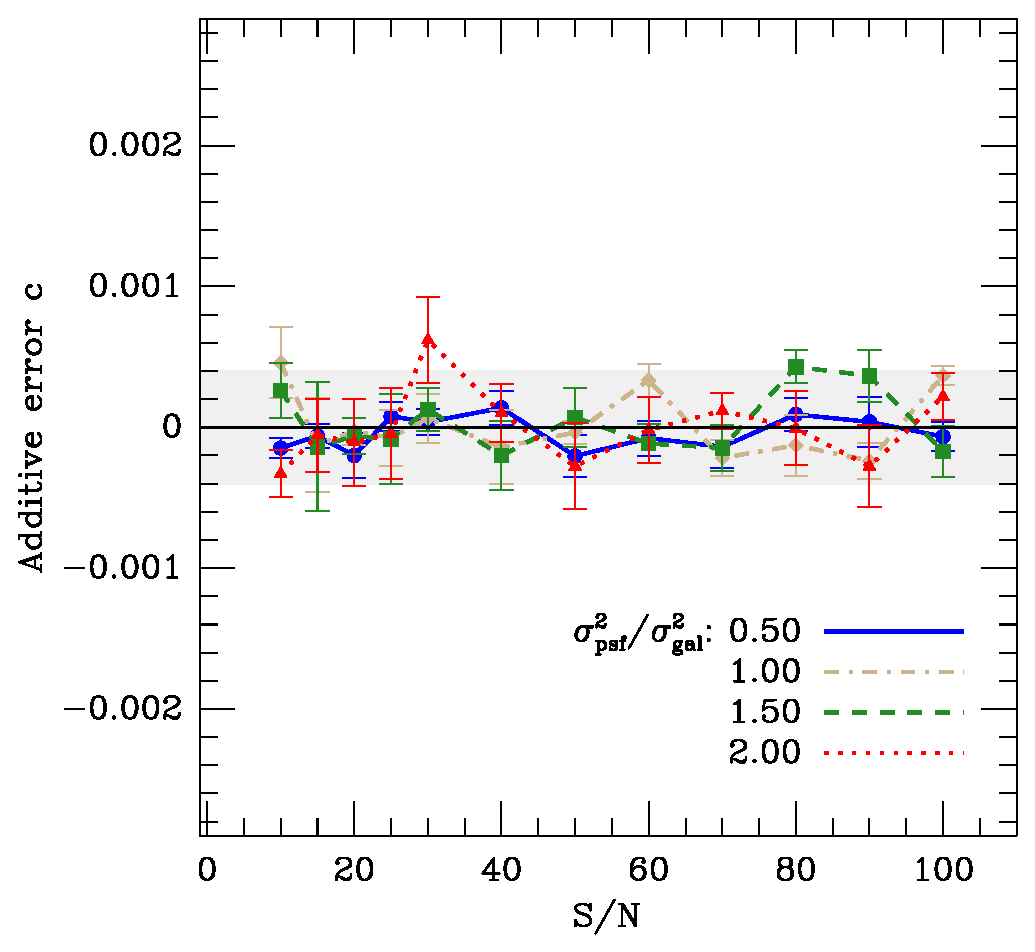
\includegraphics[scale=0.65]{figures/set-s2n-et01-c-vs-shear.eps}

 \caption{The additive error for \psf s representing atmospheric turbulence and
 exponential galaxies.  The calibration error is shown in figure
 \ref{fig:etcaliberr}.  The grey region represents the maximum additive error
 allowed by Dark Energy Survey science requirements.  For round \psf s the
 additive error is unimportant. } 

 \label{fig:etverifyadditive}
\end{figure}





\subsection{Calibration and Additive Errors for Exponential Objects and Double
Gaussian \psf s}

The double gaussian \psf\ model, based on \psf s derived from SDSS data, is
useful because it can be made elliptical.  In this section we will isolate the
calibration and additive errors in the shear recovery, as defined in the
following equation:
\begin{equation}
\langle \gamma \rangle = m\times \gamma_{true} + c
\end{equation}

XXX discuss how model is based on SDSS back in the models section


\begin{figure}[p] \centering
 \centering 
 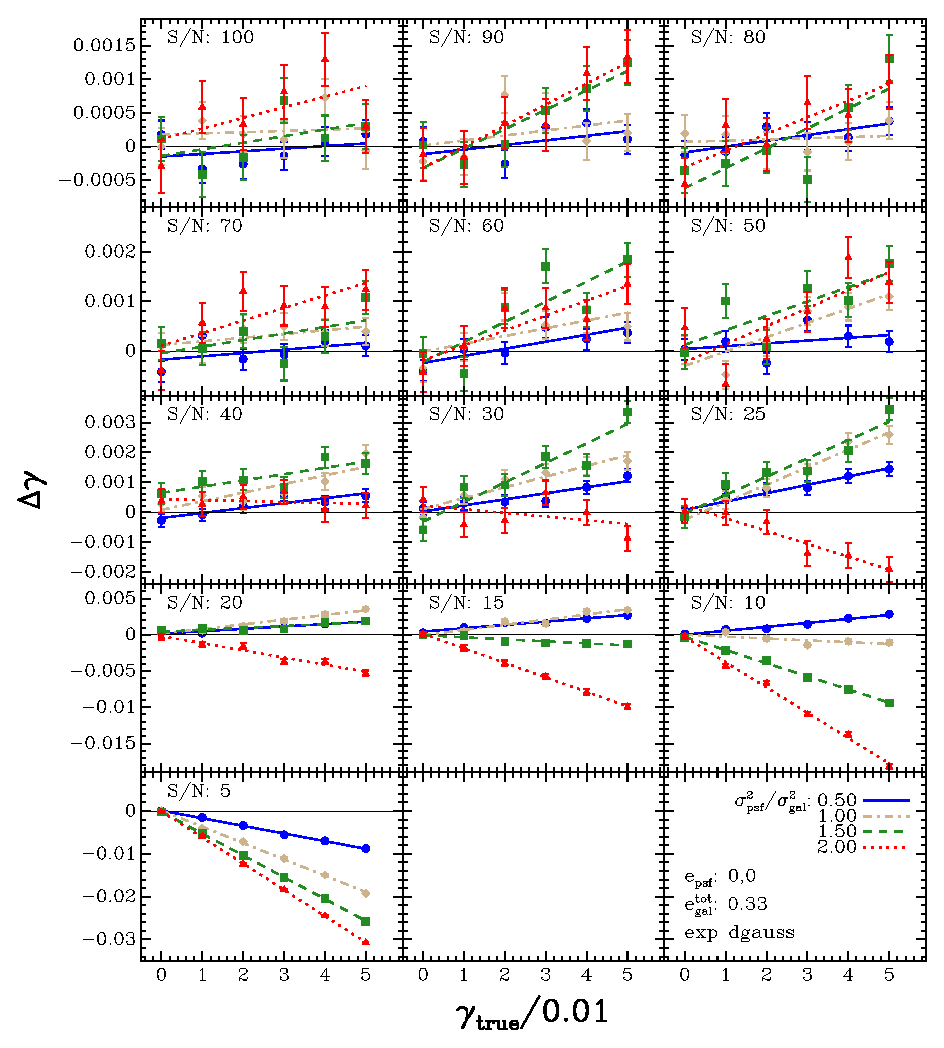
\includegraphics[scale=1.1]{figures/set-s2n-edg02-vs-shear.eps}

 \caption{Shear error vs true shear for SDSS-like round double gaussian \psf s
 and exponential galaxies.  Note the vertical scale is different for each row
 of plots.  The over-plotted curves are the best-fitting linear model.}
 \label{fig:edgdiffvsshroundpsf}

\end{figure}


\begin{figure}[t] \centering
 \centering 
 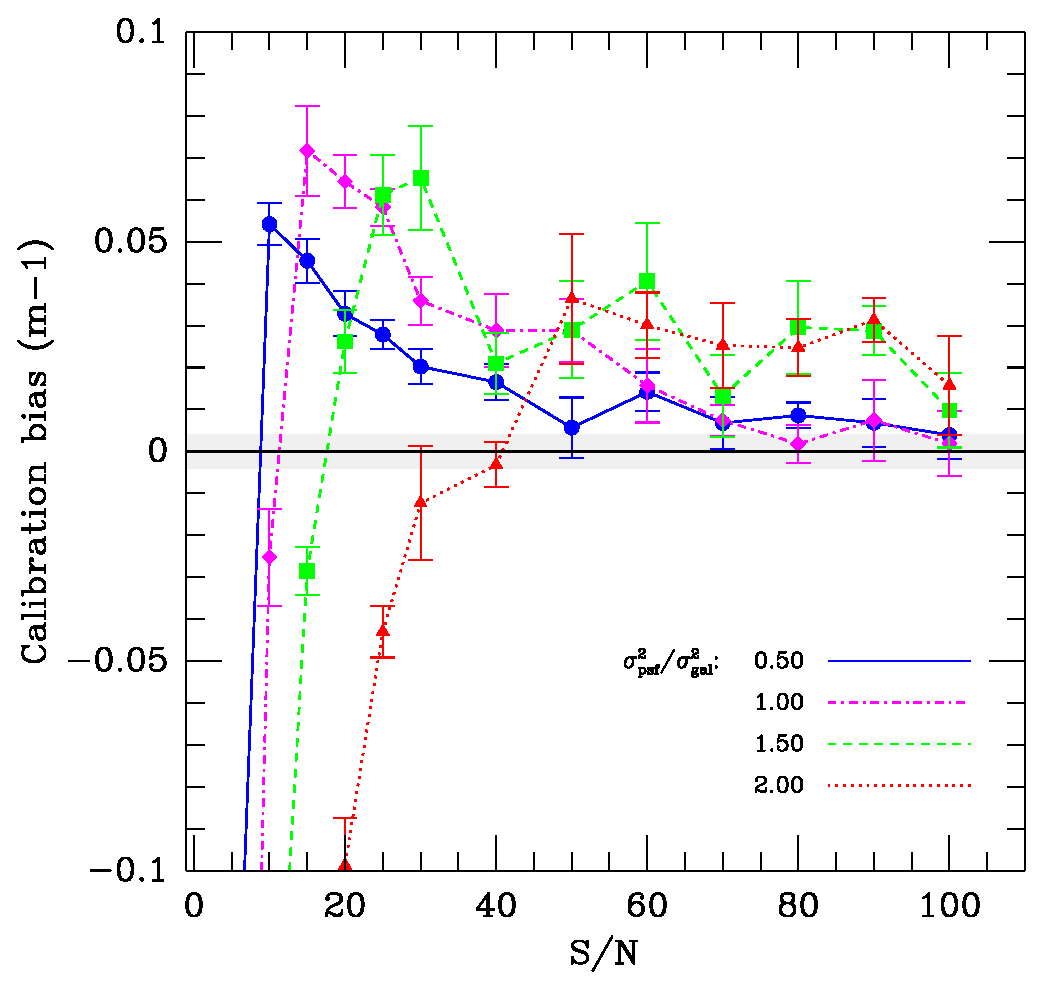
\includegraphics[scale=0.65]{figures/set-s2n-edg02-m-vs-shear.eps}

 \caption{Calibration error error as a function of matched S/N for SDSS-like
 round double gaussian \psf s and exponential galaxies.  The calibration error is
 $\Delta \gamma/\gamma = (m-1)$, where $m$ is the linear slope of the fits shown in
 Figure \ref{fig:edgdiffvsshroundpsf}.  The grey region represents the 
 maximum calibration error allowed by Dark Energy Survey science
 requirements.  The matched S/N is the maximal possible S/N measure.  Any real
 world S/N estimate will be considerably lower for these objects.} 

 \label{fig:edgcaliberr}

\end{figure}

\begin{figure}[t] \centering
 \centering 
 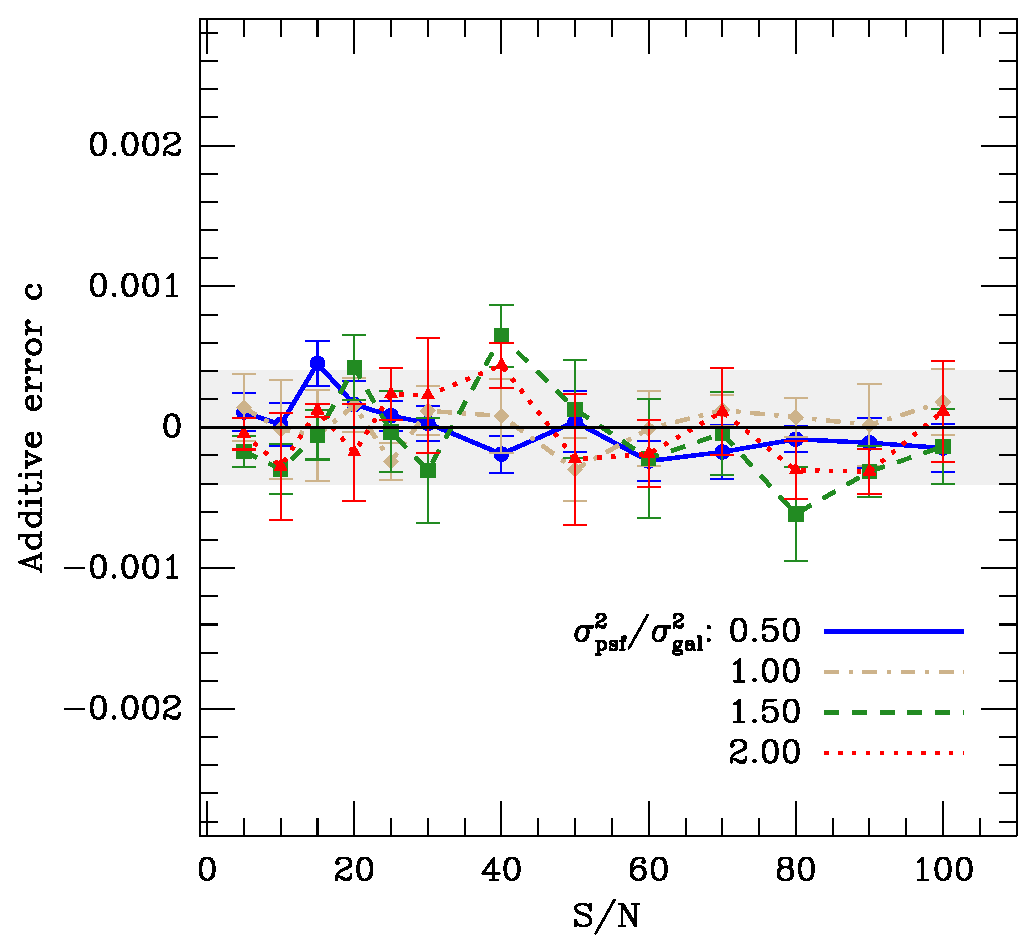
\includegraphics[scale=0.65]{figures/set-s2n-edg02-c-vs-shear.eps}

 \caption{The additive error for round double gaussian \psf s and exponential
 galaxies.  The calibration error is shown in figure \ref{fig:edgcaliberr}.
 The grey region represents the maximum additive error allowed by Dark Energy
 Survey science requirements.  For round \psf s the additive error is
 unimportant.  This plot can be compared to Figure \ref{fig:edgadderr},
 in which we show the additive error for elliptical \psf s.  } 

 \label{fig:edgverifyadditive}
\end{figure}


\subsubsection{Additive Error}

\begin{figure}[t] \centering
 \centering 
 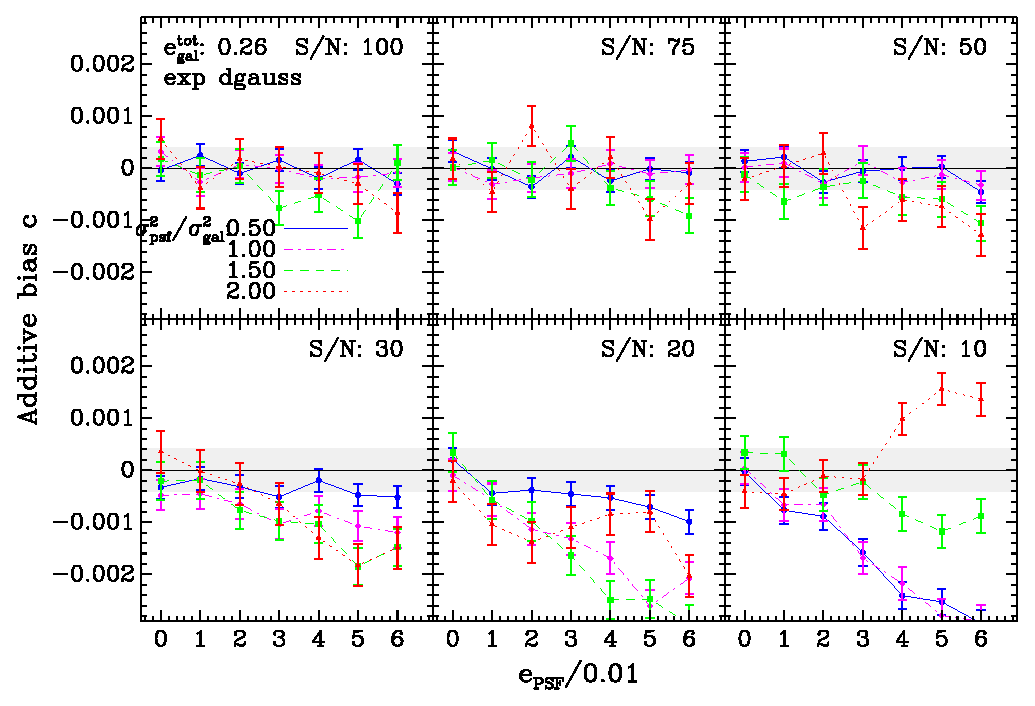
\includegraphics[scale=1]{figures/set-epsf-edg01-yr-0.003-0.003-vs-epsf.eps}

 \caption{Additive error as a function of \psf\ ellipticity and matched S/N for
 SDSS-like elliptical double gaussian \psf s and exponential galaxies.  The grey
 region represents the maximum additive error allowed by Dark
 Energy Survey science requirements.  }

 \label{fig:edgadderr}

\end{figure}




\bibliographystyle{apj}
% Bib database
\bibliography{apj-jour,astroref}

\appendix 

\section{Appendix}
\subsection{Jacobian}

The Jacobian is the set of first derivatives of model with respect
to the parameters:
\begin{equation}
J_i = \frac{\partial G}{\partial \beta_i}
\end{equation}
The jacobian can be useful in some fitting routines to help guide the descent
to best fit.

For a single Gaussian, the elements of the Jacobian can be readily
calculated.  For the parameters $x_0,y_0,\theta,T,p$ we find
\begin{eqnarray}
\frac{1}{G} \frac{\partial G}{\partial x_0}
    & = & 2 \frac{ \Dx (1-e_1) - \Dy e_2 }{T (1-e^2)} \\
\frac{1}{G} \frac{\partial G}{\partial y_0}
    & = & 2 \frac{ \Dy (1+e_1) - \Dx e_2 }{T (1-e^2)} \\
\frac{1}{G} \frac{\partial G}{\partial e_1}
  & = & \frac{e_1}{1-e^2} + \frac{\Dx^2-\Dy^2}{T (1-e^2)^2} (1-e^2 + 2 e_1^2) \\
\frac{1}{G} \frac{\partial G}{\partial e_2}
  & = & \frac{e_2}{1-e^2} + \frac{2 \Dx \Dy}{T (1-e^2)^2} (1-e^2 + 2 e_2^2) \\
\frac{1}{G} \frac{\partial G}{\partial T}
  & = & \frac{-1}{T} \left( 1 - \frac{1}{2} \X^T \M^{-1} \X  \right)  \\
\frac{1}{G} \frac{\partial G}{\partial p}
  & = & \frac{1}{p}
\end{eqnarray}

\subsection{Jacobian in the Presence of a \psf}

For $x_0,y_0,T$ and $p$, we can use the same Jacobian equations for the pre-\psf\
case, evaluated with the convolved covariance matrix. 

For $e_1$ and $e_2$ we modify the jacobians according to the following equations
\begin{eqnarray}
\frac{\partial G_o}{\partial e_1} 
 & = & \frac{\partial G_o}{\partial e_1^o} \frac{\partial e_1^o}{\partial e_1} 
    =  R \frac{\partial G_o}{\partial e_1^o}\\
\frac{\partial G_o}{\partial e_2} 
 & = & \frac{\partial G_o}{\partial e_2^o} \frac{\partial e_2^o}{\partial e_2}
    =  R \frac{\partial G_o}{\partial e_2^o}\\
R & = & \frac{T}{T + T_P} = \frac{T}{T_o}.
\end{eqnarray}
where quantities sub- or super-scripted with $o$ are convolved or ``observed''
quantities, and we have defined the resolution parameter $R$.

\end{document}

